\documentclass[letterpaper, 12pt]{math}

\usepackage{listings}
\lstset{basicstyle=\ttfamily\footnotesize,breaklines=true}
\usepackage{pgfplots}
\pgfplotsset{compat=1.8}

\title{Analysis of Algorithms}
\author{Alvin Lin (axl1439) and William Leuschner (wel2138)}
\date{August 2017 - December 2017}

\begin{document}

\maketitle

\section*{Problem 0}

\subsubsection*{Algorithm Description}
For this problem, we implemented the select linear time median algorithm to
find the median of all the points since the median point would have the smallest
total Manhattan distance to all the police cars. The integer median guarantees
us a point in the neighborhood of the optimal solution, so we simply check the
immediate points surrounding our calculated median to find the optimal solution.
This brute force check adds a small constant time to our runtime.

\subsubsection*{Argument of Correctness}
Finding the centroid (arithmetic mean of points) does not work because if there
is an outlier cop car, it will skew the Manhattan distance sums towards that
outlier, which increases the travel time from the main cluster of cop cars.
Choosing the median allows us to center the point within the cluster such that
the travel time by any car in the cluster is minimized. Note that this is true
because travel time is calculated as Manhattan distance.

\subsubsection*{Running Time Estimate}
This algorithm implements the select algorithm to do a linear time median.
\[ O(n) \]

\subsubsection*{Psuedocode}
\begin{lstlisting}
def kthSmallest(values, k):
    n = values.length
    if n <= 5:
        return bruteForceKthSmallest(values, k)
    medians = []
    j = 0
    for i = 0 to values.length by 5:
        medians[j] = bruteForceMedian(values[i:i+5])
    medianB = kthSmallest(medians)

    partition = []
    left = 0, right = n - 1
    for i = 0 to values.length:
        if values[i] < medianB:
            partition[left] = values[i]
            left += 1
        else if values[i] > medianB:
            partition[right] = values[i]
            right -= 1
    for i = left to right + 1:
        partition[i] = medianB

    pivot = left
    if pivot != right and right < n / 2:
        pivot = right

    if k < pivot:
        return kthSmallest(partition[0:pivot], k)
    else if k > pivot:
        return kthSmallest(partition[pivot + 1:n])
    return medianB

def sumManhattanDistance(coordinates, x, y):
    sum = 0
    for i = 0 to coordinates.length
        sum += |coordinates[0] - x| + |coordinates[1] - y|
    return sum

def minimizeSumDistance(coordinates):
    n = coordinates.length
    medianX = kthSmallest(coordinates[0], n / 2)
    medianY = kthSmallest(coordinates[1], n / 2)
    distance = sumManhattanDistance(coordinates, medianX, medianY)
    neighborhood = [
        [-1, 1], [-1, 0], [-1, 1]
        [0, -1], [0, 1],
        [1, -1], [1, 0], [1, 1]
    ]
    for offset in neighborhood:
        distance = min(distance, sumManhattanDistance(
            coordinates, medianX + offset[0], medianY + offset[1]))
    return distance
\end{lstlisting}

\section*{Problem 1}

\subsubsection*{Algorithm Description}
For this problem, we used a dynamic programming solution to find the maximum
number of classes that can fit into a schedule, allotting for travel time.
During each step, it computes the maximum number of classes that can be taken
from among the current subset of classes. It finds the largest previous
solution, then adds one and sets that value as the current solution, but only
if that largest solution fit before the current interval. If it was unable to
find a previous solution that fit before the current interval, then the current
solution is simply one, consisting only of the the current interval.

\subsubsection*{Argument of Correctness}
Heart of the solution:
\begin{align*}
  \texttt{S[i]} =& \text{ the maximum number of non-overlapping classes} \\
  & \text{(including travel time) from the set } a_{1}\dots a_{j}
\end{align*}
To calculate \texttt{S[i]}:
\[ \text{Let } \texttt{index} = \texttt{max(S[:i-1])} \text{ such that }
  a_{\texttt{index}}.end + \text{travel time} \le a_{\texttt{i}}.start \]
\[ \texttt{S[i]} = \texttt{S[index]} + 1 \text{ if such an index exists,
  otherwise } 1 \]
\[ \texttt{S[1] = 1} \]

\subsubsection*{Running Time Estimate}
This algorithm needs to iterate through each interval, and during each
iteration needs to find the maximum previous solution. This makes it
\( O(n^2) \).

\subsubsection*{Pseudocode}
\begin{lstlisting}
def getEndTimeWithTravel(startClass, endClass, travelTimes):
    return startClass.endTime +
        travelTimes[startClass.index][endClass.index]

def findGreatestNumberOfIntervals(intervals, travelTimes):
    intervals = heapSort(intervals, keeping track of original index)
    let solution = [] of size intervals.length
    solution[0] = 1
    for i = 1 to intervals.length:
        let current = intervals[i]
        solution[i] = 1
        for j = 0 to i:
            tmp = intervals[j]
            if solution[j] >= solution[i] and
                getEndTimeWithTravel(tmp, current, travelTimes):
                solution[i] = solution[j] + 1
    return max(solution)
\end{lstlisting}

\section*{Problem 2}
For this problem, we implemented both the recursive solution and the dynamic
programming solution.
\begin{center}
  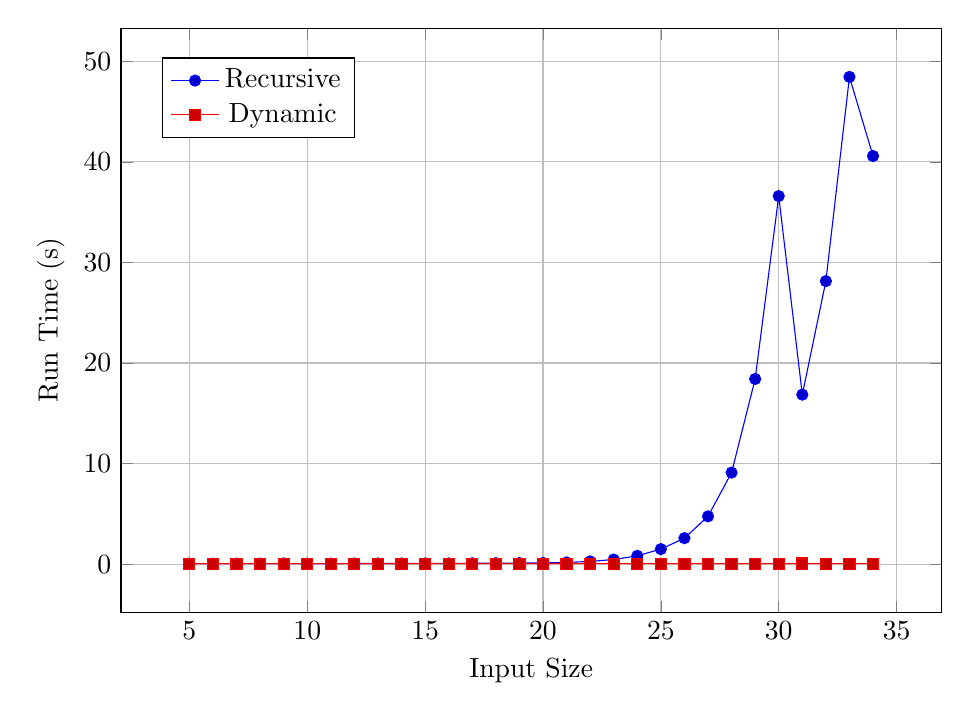
\begin{tikzpicture}
    \begin{axis}[height=9cm, width=12cm, grid=major,
        legend style={at={(0.05,0.95)},anchor=north west},
        xlabel=Input Size, ylabel=Run Time (s)
      ]
      \addplot coordinates {
        (5,0.059) (6,0.053) (7,0.056) (8,0.056) (9,0.064) (10,0.055) (11,0.055)
        (12,0.065) (13,0.068) (14,0.071) (15,0.075) (16,0.075) (17,0.087)
        (18,0.100) (19,0.110) (20,0.128) (21,0.173) (22,0.274) (23,0.460)
        (24,0.830) (25,1.497) (26,2.587) (27,4.753) (28,9.104) (29,18.413)
        (30,36.596) (31,16.855) (32,28.140) (33,48.443) (34,40.577)
      };
      \addlegendentry{Recursive}
      \addplot coordinates {
        (5,0.049) (6,0.051) (7,0.054) (8,0.050) (9,0.056) (10,0.051) (11,0.052)
        (12,0.051) (13,0.050) (14,0.052) (15,0.050) (16,0.051) (17,0.055)
        (18,0.050) (19,0.054) (20,0.052) (21,0.050) (22,0.053) (23,0.050)
        (24,0.057) (25,0.050) (26,0.050) (27,0.052) (28,0.053) (29,0.049)
        (30,0.051) (31,0.060) (32,0.052) (33,0.057) (34,0.058)
      };
      \addlegendentry{Dynamic}
    \end{axis}
  \end{tikzpicture}
\end{center}
The recursive solution is significantly slower than the dynamic programming
solution.

\subsubsection*{Recursive Solution Psuedocode}
\begin{lstlisting}
def getLongestIncreasingSubsequenceLength(sequence):
    maxLen = 0
    for i = sequence.length - 1 to 0:
        maxLen = max(incrSubseqRecursive(j, sequence).length, maxLen)
    return maxLen

def incrSubseqRecursive(index, A):
    possibilities = new max heap of arrays comparing by length
    for i = index - 1 to 0:
        if A[i] < A[index]:
            possibilities.add(incrSubseqRecursive(i, A))
    if not possibilities.empty():
        answer = possibilities.pop()
    else:
        answer = []
    answer.add(A[index])
    return answer
\end{lstlisting}
Out of curiosity, we implemented memoization into the recursive algorithm just
to see what would happen. It drastically cut down on the runtime and it was
comparable to the runtime of the dynamic programming solution, but still slower.
The main thing slowing down the recursive algorithm is simply the fact that it
has to recompute the previous solutions, unlike the dynamic programming
solution.

\section*{Problem 3}

\subsubsection*{Part 1 Psuedocode}
\begin{lstlisting}
def longestIncreasingSubsequence(sequence, start):
    if start == sequence.length - 1:
        return sequence[-1:]
    minVal = sequence[start]
    minIndex = start
    for i = start to sequence.length:
        if sequence[i] < minVal:
            minVal = sequence[i]
            minIndex = i
    return [minVal] + [findNextItem(sequence, minIndex + 1)]
\end{lstlisting}

\subsubsection*{Part 1 Running Time Estimate}
\[ O(n^2) \]

\subsubsection*{Part 1 Counterexample}
Sequence: [5, 6, 7, 8, 9, 0, 1, 2, 3] \\
Greedy Algorithm Output: [0, 1, 2, 3] \\
Optimal Solution: [5, 6, 7, 8, 9]

\subsubsection*{Part 2 Pseudocode}
\begin{lstlisting}
def longestIncreasingSubsequence(sequence, start):
    let num_loops = 0
    let subsequences = []
    for l = 0 to sequence.length:
        num_loops += 1
        let i = l
        subsequence = []
        subsequence.append(sequence[l])
        while i < sequence.length:
            num_loops += 1
            if sequence[i] < sequence[j]:
                subsequence.append(sequence[j])
                i = j
                break
            if j == sequence.length - 1:
                i = sequence.length
                break
        subsequences.append(subsequence)
    sort = sorted(subsequences by length of subsequences from max to min)
    return sort[0]
\end{lstlisting}

\subsubsection*{Part 2 Running Time Estimate}
\[ O(n^2) \]

\subsubsection*{Part 2 Counterexample}
Sequence: [1, 8, 3, 6, 5, 4, 7, 2, 9] \\
Greedy Algorithm Output: [3, 6, 7, 9] \\
Optimal Solution: [1, 3, 5, 7, 9]

\section*{Problem 4 (Our solution is wrong, please read the addendum!)}

\subsubsection*{Algorithm Description}
For this problem, we implemented a dynamic programming solution that computed
the solution by building it one interval at a time. It computes the maximum
number of possible non-overlapping interval subsets at each step and subtracts
the number of overlaps the new interval has with the current solution.

\subsubsection*{Argument of Correctness}
Given a single interval \( i_1 \), the number of non-overlapping interval
subsets \texttt{S[1]} is two, consisting of the sets \( \emptyset,\{i_1\} \).
If we add a second interval \( i_2 \) that does not overlap with \( i_1 \),
then the number of\ solutions \texttt{S[2]} is 4, or \( 2\texttt{S[1]} \),
consisting of the interval subsets \( \emptyset,\{i_1\},\{i_2\},\{i_1,i_2\} \).
If interval \( i_2 \) does overlap with \( i_1 \), then we subtract the number
of intervals it overlaps with, making the solution \( 2\texttt{S[1]}-1 \), which
consists of the intervals \( \emptyset,\{i_1\},\{i_2\} \). The solution
\texttt{S[n]} with \( n \) intervals \( i_1,i_2,\dots,i_n \) can be
generalized inductively as:
\[ \texttt{S[n]} =
  2\texttt{S[n-1]}-i_n\text{'s overlaps with previous solution} \]
where:
\[ \texttt{S[0]} = 1 \]

\subsubsection*{Running Time Estimate}
This algorithm runs a single pass through all the intervals, and on each
interval it must calculate the number of overlaps with all the intervals in
the current solution. This makes it \( O(n^2) \).

\subsubsection*{Psuedocode}
\begin{lstlisting}
def countIntervals(intervals):
  let solution = 1
  for i = 1 to intervals.length:
    solution *= 2
    for j = 1 to i:
      if interval[i] overlaps interval[j]:
        solution -= 1
  return solution
\end{lstlisting}

\subsubsection*{Addendum}
Upon further testing, we realize this solution was wrong. We tested a lot more
solutions but we were unable to come up with one that worked and satisfied
the time constraint of \( O(n^2) \).

It might be possible to fix the solution that we have, if we can somehow
calculate the following pieces of information:
\begin{enumerate}
  \item How many times each interval appears in a set
  \item How many times each interval appears in a set with every other interval
\end{enumerate}

With that information, we think it might be possible to calculate what amount
should be added to the total each time through the loop, but we aren't sure,
and we couldn't figure out a way to calculate that information that didn't
balloon our time complexity into the exponential realm.

\end{document}
